\documentclass{math}

\usepackage{forest}
\usepackage{listings}
\usepackage{tikz}
\usepackage{pgf-umlcd}
\usepackage{tikz-er2}
\usetikzlibrary{positioning}

\title{Principles of Data Management}
\author{Alvin Lin}
\date{August 2018 - December 2018}

\begin{document}

\maketitle

\section*{Entity Relationship Models}
To reiterate, when planning the logical design of the database, we need to take
into account the business need of the database and the computer scientists who
need to build the application around the database. The computer scientists
need to plan out the structure and relationships of everything in the database.

\subsection*{Entity-Relationship Model}
\textbf{Entity}: anything that is distinguishable from other objects \\
\textbf{Entity Sets}: entities that are related (share some attributes)
\[ dog = (name,DOB,gooddog,breed,color,owner) \]
\begin{center}
  \begin{tabular}{|c|c|}
    \hline
    ID & Name \\
    \hline
    1 & Harry \\
    2 & Abbey \\
    3 & Potato \\
    4 & Kali \\
    5 & Sade \\
    \hline
  \end{tabular}
  \begin{tabular}{|c|c|}
    \hline
    ID & Name \\
    \hline
    1 & Jeff \\
    2 & Pat \\
    3 & Alvin \\
    4 & Andrew \\
    \hline
  \end{tabular}
\end{center}
\textbf{Relationship Sets}: links entity sets together
\begin{itemize}
  \item Harry - 2005 - Jeff
  \item Abbey - 2005 - Pat
  \item Potato - 2016 - Alvin
  \item Kali - 2018 - Andrew
  \item Sade - 2007 - Andrew
\end{itemize}
Binary relationships link two entities, but some relationships may have 3 or
more entities. Cardinality is used in binary degree relationship sets to define
how two entity sets are linked together.
\begin{itemize}
  \item One to One
  \item One to Many
  \item Many to One
  \item Many to Many
\end{itemize}

\subsection*{Complex Attributes}
Attributes can be simple or complex, single valued or multi-valued. Single
valued attributes are things like names, which we only have one of, while
emails are multi-valued since we can have multiple. Derived attributes are
things like age, which are derived from a date of birth. The domain of an
attribute is the set of available values for an attribute. Attributes like
names and addresses can be complex attributes:
\begin{center}
  \begin{forest}
    [name
      [given]
      [middle]
      [surname]
    ]
  \end{forest} \\
  \begin{forest}
    [address
      [street
        [number]
        [name]
        [apartment]
      ]
      [city]
      [state]
      [zip]
    ]
  \end{forest}
\end{center}

\subsection*{Redundant Attributes}
\[ cat=(name,owner.name,id,age) \]
\[ owner=(id,name,address) \]
The entities in weak entity sets are not unique.
\begin{center}
  \begin{tabular}{|c|}
    \hline
    Name \\
    \hline
    Andy \\
    Bob \\
    Andy \\
    Bob \\
    \hline
  \end{tabular}
\end{center}
Cat names in this example cannot uniquely identify a cat, so we link it to a
strong entity set, which contains an identifying entity. The weak entity set is
thus dependent on strong entity set. This provides a discriminating key or
attribute that can be added to the weak entity set to make it unique.

\subsection*{ER Diagrams}
Entity Set (UML and ER diagram):
\begin{center}
  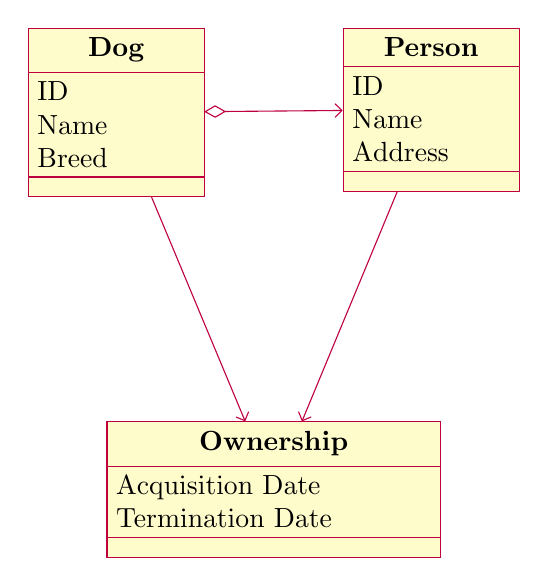
\begin{tikzpicture}
    \begin{class}[text width=2cm]{Dog}{0,0}
      \attribute{ID}
      \attribute{Name}
      \attribute{Breed}
    \end{class}
    \begin{class}[text width=2cm]{Person}{4,0}
      \attribute{ID}
      \attribute{Name}
      \attribute{Address}
    \end{class}
    \begin{class}[text width=4cm]{Ownership}{2,-5}
      \attribute{Acquisition Date}
      \attribute{Termination Date}
    \end{class}
    \aggregation{Dog}{}{}{Person}
    \unidirectionalAssociation{Dog}{}{}{Ownership}
    \unidirectionalAssociation{Person}{}{}{Ownership}
  \end{tikzpicture}
  \begin{tikzpicture}[node distance=0.5cm, every edge/.style={link}]
    \node[entity](dog){Dog};
    \node[attribute](dogname)[above left=of dog]{Name} edge (dog);
    \node[attribute](dogid)[above=of dog]{ID} edge (dog);
    \node[attribute](dogbreed)[above right=of dog]{Breed} edge (dog);

    \node[ident relationship](owns)[right=1.5cm of dog]{Owns} edge (dog);
    \node[attribute](ownsacquisition)[below left=1cm of owns]
      {Acquisition Date} edge (owns);
    \node[attribute](ownstermination)[below right=1cm of owns]
      {Termination Date} edge (owns);

    \node[entity](person)[right=5cm of dog]{Person} edge (owns);
    \node[attribute](personname)[above left=of person]{Name} edge (person);
    \node[attribute](personid)[above=of person]{Name} edge (person);
    \node[attribute](personaddress)[above right=of person]{Address} edge
      (person);
  \end{tikzpicture}
\end{center}
Dogs can also be related to other dogs, which can be represented as follows:
\begin{center}
  \begin{tikzpicture}[node distance=0.5cm, every edge/.style={link}]
    \node[entity](dog){Dog};
    \node[attribute](dogname)[above left=of dog]{Name} edge (dog);
    \node[attribute](dogid)[above=of dog]{ID} edge (dog);
    \node[attribute](dogbreed)[above right=of dog]{Breed} edge (dog);

    \node[ident relationship](owns)[right=3cm of dog]{Owns} edge[thick,double]
      node[above] {parent\_id} node[below] {pup\_id} (dog);
  \end{tikzpicture}
\end{center}

\subsubsection*{Cardinality}
\begin{itemize}
  \item 1:1
  \begin{center}
    \begin{tikzpicture}[node distance=0.5cm, every edge/.style={link}]
      \node[entity](dog){Dog};
      \node[entity](person)[right=6cm of dog]{Person};
      \node[ident relationship](owns)[right=2cm of dog]{Owns} edge[->] (dog)
        edge[->] (person);
    \end{tikzpicture}
  \end{center}
  \item 1:Many
  \begin{center}
    \begin{tikzpicture}[node distance=0.5cm, every edge/.style={link}]
      \node[entity](dog){Dog};
      \node[entity](person)[right=6cm of dog]{Person};
      \node[ident relationship](owns)[right=2cm of dog]{Owns} edge[->] (dog)
        edge (person);
    \end{tikzpicture}
    \begin{tikzpicture}[node distance=0.5cm, every edge/.style={link}]
      \node[entity](dog){Dog};
      \node[entity](person)[right=6cm of dog]{Person};
      \node[ident relationship](owns)[right=2cm of dog]{Owns}
        edge node[above]{0..*} (dog)
        edge[double] node[above]{1..1} (person);
    \end{tikzpicture}
  \end{center}
  A person has exactly one dog and every dog has zero or more owners.
  \begin{center}
    \begin{tikzpicture}[node distance=0.5cm, every edge/.style={link}]
      \node[entity](dog){Dog};
      \node[entity](person)[right=6cm of dog]{Person};
      \node[ident relationship](owns)[right=2cm of dog]{Owns} edge[double] (dog)
        edge[->] (person);
    \end{tikzpicture}
  \end{center}
  Every dog has exactly one owner and every owner has zero or more dogs.
  \item Many:1
  \begin{center}
    \begin{tikzpicture}[node distance=0.5cm, every edge/.style={link}]
      \node[entity](dog){Dog};
      \node[entity](person)[right=6cm of dog]{Person};
      \node[ident relationship](owns)[right=2cm of dog]{Owns} edge (dog)
        edge[->] (person);
      \path (person) edge[bend right,->] node[above] {many} (dog);
      \path (dog) edge[bend right,->] node[below] {one} (person);
    \end{tikzpicture}
  \end{center}
\end{itemize}
A single line implies a 0..N relationship in that one thing can have 0 or more
of another object, while a double line implies 1..N which implies a one or more
relationship.

\subsubsection*{Complex Attributes}
UML:
\begin{center}
  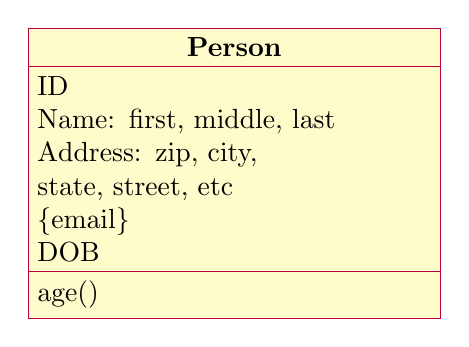
\begin{tikzpicture}
    \begin{class}[text width=5cm]{Person}{0,0}
      \attribute{ID}
      \attribute{Name: first, middle, last}
      \attribute{Address: zip, city, state, street, etc}
      \attribute{\{email\}}
      \operation{age()}
      \attribute{DOB}
    \end{class}
  \end{tikzpicture}
\end{center}
For the accompanying Chen ER diagram, multi-valued attributes like email are
double circled, while derived attributes like age are dotted.
\begin{center}
  \begin{tikzpicture}[node distance=0.5cm, every edge/.style={link}]
    \node[entity](person){Person};
    \node[attribute](id)[above=of person]{ID} edge (person);

    \node[attribute](name)[above right=of person]{Name} edge (person);
    \node[attribute](first)[above left=1cm of name]{First} edge (name);
    \node[attribute](middle)[above=of name]{Middle} edge (name);
    \node[attribute](last)[above right=1cm of name]{Last} edge (name);

    \node[attribute](address)[right=of person]{Address} edge (person);
    \node[attribute](zip)[above right=of address]{ZIP} edge (address);
    \node[attribute](street)[right=of address]{Street} edge (address);
    \node[attribute](number)[above right=of street]{Number} edge (street);
    \node[attribute](name)[right=of street]{Name} edge (street);
    \node[attribute](apartment)[below right=of street]{Apartment} edge (street);
    \node[attribute](etc)[below right=of address]{...} edge (address);

    \node[derived attribute](age)[below=1cm of person]{Age} edge (person);
    \node[multi attribute](email)[below left=of person]{Email} edge (person);
    \node[attribute](dob)[below right=of person]{DOB} edge (person);
  \end{tikzpicture}
\end{center}
Sometimes, weak entity sets must rely on another entity in order to be uniquely
identified. For example:
\begin{center}
  \begin{tikzpicture}[node distance=0.5cm, every edge/.style={link}]
    \node[entity](employee){Employee};
    \node[attribute](id)[below=of employee]{ID} edge (employee);

    \node[ident relationship](hasa)[right=of employee]{Has A} edge (employee);

    \node[entity,double](child)[right=of hasa]{Child} edge[total] (hasa);
    \node[derived attribute](name)[above right=of child]{Name} edge (child);
    \node[derived attribute](dob)[below right=of child]{DOB} edge (child);
  \end{tikzpicture}
\end{center}
If there are two children (of two employees) with the same name and date of
birth, then they are reliant on their relationship with the employee and the
employee's ID in order to be uniquely identified.

\subsubsection*{Reduction into Tables}
\begin{center}
  \begin{tikzpicture}[node distance=0.5cm, every edge/.style={link}]
    \node[entity](dog){Dog};
    \node[attribute](dogname)[above left=of dog]{Name} edge (dog);
    \node[attribute](dogid)[above=of dog]{ID} edge (dog);
    \node[attribute](dogbreed)[above right=of dog]{Breed} edge (dog);

    \node[ident relationship](owns)[right=1.5cm of dog]{Owns} edge (dog);

    \node[entity](person)[right=5cm of dog]{Person} edge (owns);
    \node[attribute](personname)[above left=of person]{Name} edge (person);
    \node[attribute](personid)[above=of person]{ID} edge (person);
    \node[attribute](persondob)[above right=of person]{DOB} edge (person);
  \end{tikzpicture}
\end{center}
\begin{align*}
  Person &= (\textbf{id}, name, DOB) \\
  Dog &= (\textbf{id}, name, breed) \\
  owns &= (\textbf{person.id}, \textbf{dog.id})
\end{align*}
While the primary key of people and dogs can just be their id, the ``owns''
table's primary key is both the person and dog id of the association in order
to prevent ambiguity.
\begin{center}
  \begin{tikzpicture}[node distance=0.5cm, every edge/.style={link}]
    \node[entity](person){Person};
    \node[attribute](id)[above=of person]{ID} edge (person);

    \node[attribute](name)[above right=of person]{Name} edge (person);
    \node[attribute](first)[above left=1cm of name]{First} edge (name);
    \node[attribute](middle)[above=of name]{Middle} edge (name);
    \node[attribute](last)[above right=1cm of name]{Last} edge (name);

    \node[attribute](address)[right=of person]{Address} edge (person);
    \node[attribute](zip)[above right=of address]{ZIP} edge (address);
    \node[attribute](street)[right=of address]{Street} edge (address);
    \node[attribute](number)[above right=of street]{Number} edge (street);
    \node[attribute](name)[right=of street]{Name} edge (street);
    \node[attribute](apartment)[below right=of street]{Apartment} edge (street);
    \node[attribute](etc)[below right=of address]{...} edge (address);

    \node[derived attribute](age)[below=1cm of person]{Age} edge (person);
    \node[multi attribute](email)[below left=of person]{Email} edge (person);
    \node[attribute](dob)[below right=of person]{DOB} edge (person);
  \end{tikzpicture}
\end{center}
\begin{align*}
  Person &= (\textbf{id}, dob, name\_first, name\_middle, name\_last, zip, \\
  & state, city, street\_number, street\_name, apartment) \\
  Email &= (\textbf{person\_id}, \textbf{email\_address})
\end{align*}
In this example, age is a derived attribute, so it is not included in the table,
and email is a multi-valued attribute, so we have a separate table for it. This
table's primary key is both the person id and their email address.
\begin{center}
  \begin{tikzpicture}[node distance=0.5cm, every edge/.style={link}]
    \node[entity](dog){Dog};
    \node[attribute](dogname)[above left=of dog]{Name} edge (dog);
    \node[attribute](dogid)[above=of dog]{ID} edge (dog);
    \node[attribute](dogbreed)[above right=of dog]{Breed} edge (dog);

    \node[ident relationship](owns)[right=1.5cm of dog]{Owns} edge[total] (dog);

    \node[entity](person)[right=5cm of dog]{Person} edge (owns);
    \node[attribute](personname)[above left=of person]{Name} edge (person);
    \node[attribute](personid)[above=of person]{ID} edge (person);
    \node[attribute](persondob)[above right=of person]{DOB} edge (person);
  \end{tikzpicture}
\end{center}
\begin{align*}
  Dog &= (\textbf{dog\_id}, dog\_name, breed, person\_id, person\_name) \\
\end{align*}
In this example with total participation, a dog must have one and only one
owner, while a person may have multiple dogs. Thus, the dog table can include
the person id.
\begin{center}
  \begin{tikzpicture}[node distance=0.5cm, every edge/.style={link}]
    \node[entity](dog){Dog};
    \node[attribute](dogname)[above left=of dog]{Name} edge (dog);
    \node[attribute](dogid)[above=of dog]{ID} edge (dog);
    \node[attribute](dogbreed)[above right=of dog]{Breed} edge (dog);

    \node[ident relationship](owns)[right=1.5cm of dog]{Owns} edge[->] (dog);

    \node[entity](person)[right=5cm of dog]{Person} edge[<-] (owns);
    \node[attribute](personname)[above left=of person]{Name} edge (person);
    \node[attribute](personid)[above=of person]{ID} edge (person);
    \node[attribute](persondob)[above right=of person]{DOB} edge (person);
  \end{tikzpicture}
\end{center}
\begin{align*}
  Person &= (\textbf{id}, name, dob, \textbf{dog\_id}, dog\_name)
\end{align*}
If we decide that the relationship must be one to one, then a person may have
zero or one dogs, and a dog may have zero or one owners. Without total
participation, both the dog id and the person's id must be part of the primary
key of the table.

\subsubsection*{Ternary Relationships}
Because this can be ambiguous, we only allow for one arrow indicating ownership.
\begin{center}
  \begin{tikzpicture}[node distance=0.5cm, every edge/.style={link}]
    \node[entity](instructor){Instructor};
    \node[ident relationship](have)[right=of instructor]{} edge (instructor);
    \node[entity](student)[right=of have]{Student} edge[<-] (have);
    \node[entity](project)[above=of have]{Project} edge (have);
  \end{tikzpicture}
\end{center}
Often, it is better to reduce this to multiple binary relationships:
\begin{center}
  \begin{tikzpicture}[node distance=0.5cm, every edge/.style={link}]
    \node[entity](project){Project};
    \node[ident relationship](workedon)[below left=of project]{Worked On}
      edge (project);
    \node[ident relationship](advised)[below right=of project]{Advised}
      edge (project);
    \node[entity](student)[below left=of workedon]{Worked On} edge (workedon);
    \node[entity](instructor)[below right=1cm of advised]{Advised} edge
      (advised);
    \node[ident relationship](workedwith)[right=2cm of student]{Worked With}
      edge (student) edge (instructor);
  \end{tikzpicture}
\end{center}
Sometimes, we may use a different notation for a use case like this:
\begin{center}
  \begin{tikzpicture}[node distance=0.5cm, every edge/.style={link}]
    \node[entity](person){Person};
    \node[attribute](id)[above left=1cm of person]{ID} edge (person);
    \node[attribute](fname)[above=1cm of person]{First name} edge (person);
    \node[attribute](lname)[above right=1cm of person]{Last name} edge (person);

    \node[ident relationship](isa)[below=of person]{Is A} edge (person);

    \node[entity](student)[below left=of isa]{Student} edge[->] (isa);
    \node[attribute](debt)[above left=of student]{Debt} edge (student);

    \node[entity](employee)[below right=of isa]{Employee} edge[->] (isa);
    \node[attribute](salary)[above right=of employee]{Salary} edge (employee);
    \node[entity](salaried)[below left=of employee]{Salaried} edge[->]
      (employee);
    \node[attribute](age)[below=of salaried]{Age} edge (salaried);
    \node[entity](hourly)[below right=of employee]{Hourly} edge[->] (employee);
    \node[attribute](hours)[below=of hourly]{Hours} edge (hourly);
  \end{tikzpicture}
\end{center}
When reducing this to tables we have a few options:
\begin{enumerate}
  \item Take all the attributes from every level, and make entities with lower
    levels have a higher level primary key.
  \begin{align*}
    Person &= (ID, fname, lname) \\
    Student &= (ID, debt) \\
    Employee &= (ID, salary) \\
    Salaried &= (ID, age) \\
    Hourly &= (ID, hours)
  \end{align*}
  \item Create entity ``leafs'', grabbing attributes from higher levels.
  \begin{align*}
    Student &= (ID, fname, lname, debt) \\
    Hourly &= (ID, fname, lname, salary, hours) \\
    Salaried &= (ID, fname, lname, salary, age) \\
  \end{align*}
  \item Throw everything into one table (which is usually a bad choice).
  \begin{align*}
    Person &= (ID, fname, lname, salary, hours, age, debt)
  \end{align*}
\end{enumerate}
The concept of total and partial completeness still exists for these
relationships. With total completeless, the higher level MUST belong to the
lower level. This would be represented as:
\begin{center}
  \begin{tikzpicture}[node distance=0.5cm, every edge/.style={link}]
    \node[entity](person){Person};
    \node[ident relationship](isa)[below=1.5cm of person]{Is A} edge[double,->]
      (person);
  \end{tikzpicture}
\end{center}
With the salaried/hourly employee dichotomy, total completeness is implied
because they are disjoint categories of employees.

\subsubsection*{Entity vs Attribute}
Sometimes, we may make a choice like so:
\begin{center}
  \begin{tikzpicture}[node distance=0.5cm, every edge/.style={link}]
    \node[entity](person){Person};
    \node[attribute](id)[left=of person]{ID} edge (person);
    \node[multi attribute](email)[above=of person]{Email} edge (person);

    \node[ident relationship](born)[right=of person]{Born} edge (person);

    \node[entity](birthinfo)[right=of born]{Birth Info} edge[<-] (born);
    \node[attribute](birthid)[above=of birthinfo]{ID} edge (birthinfo);
    \node[attribute](dob)[right=of birthinfo]{DOB} edge (birthinfo);
  \end{tikzpicture}
\end{center}
This has the advantage of reducing some redundancy as multiple people can share
entries in the birth info table. For complex attributes, it may sometimes be
prudent to separate out the attribute into its own entity. As another example:
\begin{center}
  \begin{tikzpicture}[node distance=0.5cm, every edge/.style={link}]
    \node[entity](student){Student};
    \node[ident relationship](workedon)[right=of student]{Worked On} edge
      (student);
    \node[attribute](startdate)[above left=of workedon]{Start Date} edge
      (workedon);
    \node[attribute](enddate)[above right=of workedon]{End Date} edge
      (workedon);
    \node[entity](project)[right=of workedon]{Project} edge (workedon);
  \end{tikzpicture}
\end{center}

\begin{center}
  You can find all my notes at \url{http://omgimanerd.tech/notes}. If you have
  any questions, comments, or concerns, please contact me at
  alvin@omgimanerd.tech
\end{center}

\end{document}
